\documentclass[a4paper, twocolumn]{article}
\usepackage{CJKutf8}
\usepackage[sc]{mathpazo} % Use the Palatino font
\usepackage[T1]{fontenc} % Use 8-bit encoding that has 256 glyphs
\linespread{1.2} % Line spacing - Palatino needs more space between lines
\usepackage{microtype} % Slightly tweak font spacing for aesthetics

\usepackage[english]{babel} % Language hyphenation and typographical rules

\usepackage[hmarginratio=1:1,top=32mm,left=20mm,right=20mm,columnsep=20pt]{geometry} % Document margins
\usepackage[hang, small,labelfont=bf,up,textfont=it,up]{caption} % Custom captions under/above floats in tables or figures
%\usepackage{booktabs} % Horizontal rules in tables

\usepackage{lettrine} % The lettrine is the first enlarged letter at the beginning of the text

\usepackage{enumitem} % Customized lists
\setlist[itemize]{noitemsep} % Make itemize lists more compact

\usepackage{abstract} % Allows abstract customization
\renewcommand{\abstractnamefont}{\normalfont\itshape\bfseries} % Set the "Abstract" text to bold
\renewcommand{\abstracttextfont}{\normalfont} % Set the abstract itself to small italic text

\usepackage{titlesec} % Allows customization of titles
\renewcommand\thesection{\Roman{section}} % Roman numerals for the sections
\renewcommand\thesubsection{\roman{subsection}} % roman numerals for subsections
\titleformat{\section}[block]{\large\scshape\centering}{\thesection.}{1em}{} % Change the look of the section titles
\titleformat{\subsection}[block]{\large}{\thesubsection.}{1em}{} % Change the look of the section titles

\usepackage{fancyhdr} % Headers and footers
\pagestyle{fancy} % All pages have headers and footers
\fancyhead{} % Blank out the default header
\fancyfoot{} % Blank out the default footer
\fancyhead[C]{
	\begin{CJK}{UTF8}{gbsn}
	《计算机视觉》课程项目报告
	\end{CJK}}
\fancyfoot[RO,LE]{\thepage} % Custom footer text
\usepackage{titling} % Customizing the title section

\usepackage{hyperref} % For hyperlinks in the PDF
\hypersetup{hidelinks}

\usepackage{graphicx}
\renewcommand{\normalsize}{\fontsize{10.5pt}{\baselineskip}\selectfont}
%----------------------------------------------------------------------------------------
%	TITLE SECTION
%----------------------------------------------------------------------------------------

\setlength{\droptitle}{-4\baselineskip} % Move the title up

\pretitle{\begin{center}\Huge\bfseries} % Article title formatting
	\posttitle{\end{center}} % Article title closing formatting
\title{基于编码特征的二维码检测方法研究} % Article title
\author{%
	\textsc{刘阳 13307130167} \\[1ex] % Your name
	\normalsize 复旦大学 计算机学院 \\ % Your institution
}
\date{} % Leave empty to omit a date

%----------------------------------------------------------------------------------------

\begin{document}
\begin{CJK}{UTF8}{gbsn}
	% Print the title
	\maketitle
	
	%----------------------------------------------------------------------------------------
%		ARTICLE CONTENTS
	%----------------------------------------------------------------------------------------
	\section{摘要}

	\section{关键词}
	\section{引言}
\subsection{问题陈述}
本报告主要依据二维码的编码特点,研究二维码的检测方法。
虽然二维码的编码规范有助于实现快速检测的算法,但是真实场景中,二维码取景时往往伴随着光照不足,摄像设备分辨率低,图像倾斜,变形,扭曲,甚至部分被遮挡的情况。
而我们不单单满足于规范二维码的检测,而是要挑战复杂摄像条件下二维码的检测。\\
具体挑战分为:1. 光照不足引起的图像二值化效果不理想问题,2.摄像设备分辨率低引起的图像边缘检测问题,3.二维码取景时的噪声问题,4.二维码定位模块的位置检测问题,5.多二维码分割问题,6.变形图像的变换问题。

\subsection{应用场合}
由于二维码具有信息编码密度高,信息类型丰富,版本众多,易于定制化等等特点,二维码在生活生产中具有广泛的应用场景。而实现在复杂场景下的二维码检测方法,则能够帮助二维码应用到更多场合中,如光照不足的矿业,使用低端摄像设备的流水线生产行业等等。

\subsection{研究历史}
针对二维码检测中的主要环节,我们依次介绍相关方面的研究历史。

\subsubsection{二维码图像的二值化问题}
应用场景中采集的二维码图像是RGB模式的三色图像,为了减少之后图像处理的计算量,加速二维码检测算法,我们首先需要将二维码图像转化为灰度图。
摄像设备在不同光照条件下采集到的图像灰度水平不同。对于二维码来说,明确地分辨出对应像素点是黑还是白,是便于之后二维码定位的关键步骤。因此能否有效地将二维码二值化是一个很重要的问题。\\
对图像进行二值化分为全局阈值方法和局部阈值方法。\\
全局阈值方法中最简单最通用的方法是固定阈值,将某一灰度以下的像素全部设为黑色,而其他像素设为白色。
而另一种效果较好的方法是找出图像中的最大值和最小值,然后将中点作为阈值。典型的方法是OTSU算法(最大类间方差法)。OTSU的中心思想是最好的阈值应该使得被阈值分开的两组的方差加权和达到最大\cite{1}。而Kittler的实验\cite{2}也表明,当图像灰度直方图呈现双峰时,使用最大类间方差法效果较好,而当图像中目标与背景的大小之比较小时,该方法的效果较差。\\
Bernsen是局部阈值方法的典型算法。它通过定义考察点的邻域,并由邻域计算模板来实现考察点灰度与邻域的比较,它较适合解决光照不均的问题,而影响二维码图像读取的最严重问题也正是光照不均问题,但Bernsen算法也有速度慢,对干扰比较敏感和易导致伪影的缺点,特别是伪影问题,如果伪影现象严重,不仅会给图像带来大量的干扰,严重的还会导致后续译码的失败\cite{3}\cite{4}\cite{5}。这是因为Bernsen算法以局部窗口内最大、最小值作为考察点的域值。当局部窗口内无目标经过时,个别噪声点就会引起阈值的剧烈变化。另外,背景灰度的非均匀性也可能影响到局部阈值。\\
Shih-Chang Hsia等人提出一种自适应的补偿背景光的方法\cite{6},可以将其用于二维码二值化前的预处理。

\subsubsection{倾斜纠正}
倾斜的二维码需要倾斜纠正。根据图像边缘可以获得二维码的倾斜角度,然后将图像旋正。边缘是图像最基本的特征,所谓边缘是指图像周围像素灰度有阶跃变化或屋顶状变化的像素的集合。经典的边缘检测算法是构造对像素灰度级阶跃变化敏感的微分算子,常用的边缘提取算子有Sobel边缘算子,Laplacian算子,Canny算子等等\cite{7}。边缘检测算法得到的往往是断续的、不完整的结构信息,对噪声较为敏感。为了有效抑制噪声,在作边缘检测前,必须对图像进行平滑处理。另外,使用微分算子进行边缘检测的计算量仍然很大。\\
在二维码中,检测倾斜角度应用较多的是Hough变换和Radon变换两种方法。\\
Hough变换:利用Hough变换计算倾斜图像角度是广泛使用的一种方法。Hough变换把直线上的点的坐标转换到过点的直线的系数域,对于直线信息明显且干扰小的图像,Hough变换效果比较明显\cite{7}。但在实际使用中,会受到图像周边因素的干扰,或者条码线条比较粗,Hough变换会出现峰值扩散。对高噪声下的二维码,Hough变换效果不佳。并且Hough变换的计算量较大,不能满足实时译码的需要。\\
Radon变换:Radon变换是一种将数字图像变换为在某一指定角度射线方向上投影的方法\cite{7}。在一定范围内对二维码边缘图像求出最大积分的值,然后求出对应于最大积分值的角度,即是条码的旋转角度。该算法能够提高识别的抗噪性,,但是运算速度受到条码旋转角度范围和步进角度影响。\\
不论是Hough变换还是Radon变换,中心思想都是先计算图像倾斜的角度,然后使用点运算将图像旋转纠正。对于仅发生倾斜而没有发生形变的条码纠正效果较好,但对于采集图像过程中易发生的形变问题就束手无策了。

\subsubsection{条码定位}

	\section{二维码结构和编码}
二维码可以分为行排式(堆叠式)二维码和矩阵式二维码。\\
行排式/堆叠式二维码形态上是由多行短截的一维条码堆叠而成。
行排式/堆叠式二维码的编码原理是建立在一维条码基础之上的,按需要堆积成多行。它在编码设计、校验原理、识读方式等方面继承了一维条码的一些特点,识读设备与条码印刷和一维条码技术兼容。
代表性的行排式二维码有Code49,Code 16k,PDF417等。\\
矩阵式二维码以矩阵的形式组成,在矩阵相应元素位置上用“点”表示二进制的“1”,用“空”表示二进制的“0”,有“点”和“空”的排列组成信息编码。
矩阵式二维码是一种原理和方法与行排式二维码完全不同的条码系统。
行排式二维码和一维条码的编码都是对条码黑白相间条空的宽度进行调制,而矩阵码是对条码整个编码区域内的点进行编码,所以矩阵码有比行排式二维码高得多的信息密度。
行排式二维码只是在形式上像二维码,而本质上完全属于一维条码,所以有人也称行排式二维码为1.5维条码,而矩阵码才是真正的二维条码。
代表性的矩阵式二维码有QR Code,Code One,Data Matrix等。\\
由于QR码在日常生活中应用最为广泛,本篇报告着重研究QR码的检测。

\subsection{QR码的结构}
QR码由正方形方格组成,组成正方形阵列。
它由编码区域和包括定位模块,分隔线,修正模块,对齐模块在内的功能图形组成。
功能图形不能用于数据编码。
符号的四周由空白区域包围。
QR码的编码示意如图\ref{fig:structure1}。

\begin{figure}[h]
\centering
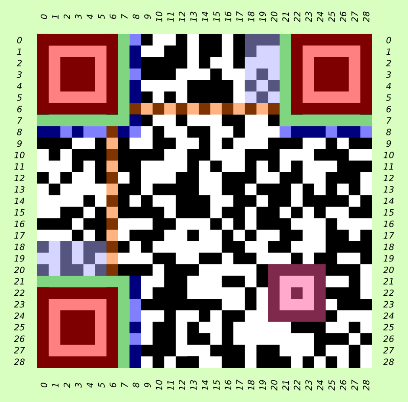
\includegraphics[width=0.9\linewidth]{structure1}
\caption[QR码结构]{QR码结构}
\label{fig:structure1}
\end{figure}

QR码的最小组成单元是方格,白色代表二进制“0”,黑色代表二进制“1”,如图\ref{fig:structure2}定义。

\begin{figure}[h]
\centering
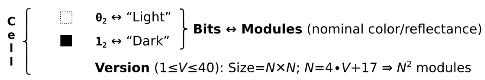
\includegraphics[width=0.9\linewidth]{structure2}
\caption[cell]{QR码的最小单元}
\label{fig:structure2}
\end{figure}

图\ref{fig:structure1}中的功能图形分为分隔线,定位模块,对齐模块,修正模块等,如图\ref{fig:structure3}所示。

\begin{figure}[h]
\centering
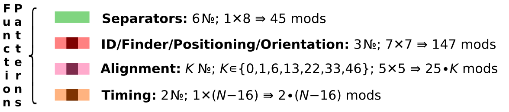
\includegraphics[width=0.9\linewidth]{structure3}
\caption[functional]{QR码的功能图形}
\label{fig:structure3}
\end{figure}

图\ref{fig:structure1}中的编码区域分为格式信息,版本信息和数据内容,如图\ref{fig:structure4}所示。

\begin{figure}[h]
\centering
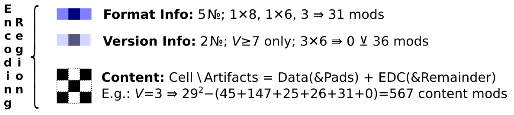
\includegraphics[width=0.9\linewidth]{structure4}
\caption[content]{QR码的编码区域}
\label{fig:structure4}
\end{figure}

各个模块的具体说明如下:\\ \\
(1).符号版本和规格\\
QR码符号共有40种规格,分别是版本1~版本40。版本1的规格为21*21个方格,版本2的规格为25*25个方格。以此类推,版本N的规格为$ (21+4*(N-1))^2 $个方格。\\
(2).定位模块\\
定位模块包括3个位置相同的位置探测图形,分别位于二维码图形的左上角、右上角和左下角。每个位置探测图形可以看作是由3个重叠的同心正方形组成,分别为7*7个黑色方格、5*5个白色方格,3*3个黑色方格。位置探测图形的模块宽度比为$ 1:1:3:1:1 $。而在二维码其他地方遇到类似图形的可能性极小。因此,识别出组成定位模块的3个位置探测图形,就可以明确地确定二维码的位置和方向。这也是本次研究的核心思想:\textbf{利用二维码的编码特点做二维码的检测}。\\
(3).分隔线\\
每个定位模块和编码区域之间有宽度为1个方格的分隔线,全部由白色方格组成。\\
(4).修正模块\\
修正模块是垂直和水平方向一个方格宽的一列和一行,由黑色白色方格交替组成,其开始和结尾都是黑色方格。\\
(5).对齐模块\\
对齐模块可看作是3个重叠的同心正方形组成,由5*5个黑色方格、3*3个白色方格以及位于中心的一个黑色方格组成。对齐模块的数量由QR码的版本号决定,版本2及以上的二维码都有对齐模块。\\
(6).编码区域\\
编码区域包括数据内容,纠错码,版本信息和格式信息。\\
(7).空白区\\
空白区为环绕在二维码四周的4个方格宽的区域,一般为白色。

\subsection{QR码的编码}
由于QR码的编码对于检测二维码几乎没有帮助,所以在这里只是简单介绍。\\
QR码通过RS码(Reed-Solomon)编码来实现纠错。在各块的纠错码字生成后,把数据码字和纠错码字排列成最终位流序列。\\
QR码编码还需要一个掩模的步骤。掩模的目的是均衡地安排黑色与白色模块,以及尽可能地避免位置探测图形的位图“1011101”出现在二维码的其他区域。
掩模不能用于功能图形,用多个矩阵图形连续地对已知的编码区域的模块图形(格式信息和版本信息除外)进行异或操作。对不同掩模图形的结果计分,选择得分最低的掩模方案。\\
最后将格式信息和版本信息放入QR码的相应区域,完成QR码的编码。\\
整个过程的示意图\ref{fig:encoding1}如下。

\begin{figure}[h]
\centering
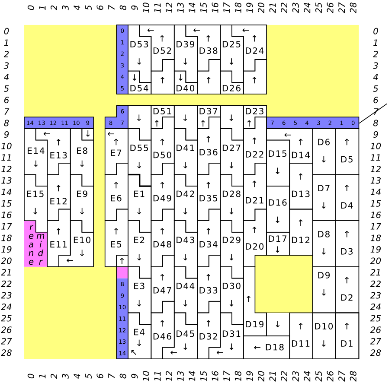
\includegraphics[width=0.9\linewidth]{encoding1}
\caption[encoding]{QR码的编码顺序}
\label{fig:encoding1}
\end{figure}

其中“D”开头的格子表示数据段,“E”开头的格子表示纠错段,浅紫色区域表示格式信息和版本信息。

	\section{方法}
	\section{实验和讨论}
\subsection{实验设置}
实验的方式主要采用的是绘制出检测框,作人眼的评价,同时监测算法执行的时间。
\subsection{评价指标}
(1).二维码检测的准确率:在原始图像上绘制出检测方法的结果,评价检测框和真实二维码位置的重叠率。\\
(2).二维码检测的效率:监测二维码检测算法执行的时间
\subsection{实验结果}
(1).在准确率上,基本方法只能识别单个方正的二维码。对于多个二维码的情况,则全部误检。
而改进方法能够识别所有的测试图像,包括多个二维码并存,或残缺二维码的图像,以及变形的图像。\\
(2).在效率上,对于同一张二维码图像,基本方法大致比改进方法快了三倍。
\subsection{比较和讨论}
从上述实验的结果看,大致和我们在方法优缺点比较时的结论一致。\\
从准确度上讲,改进方法针对基本方法在检测上的不足做了专门的优化,检测的性能必然比基本方法好,能够处理的复杂情况也比基本方法多。
另一方面,正是因为改进方法增强了检测能力,相应地就要付出检测时间上的代价,比基本方法慢两三倍也是很正常的。总的来说,即使有时间上的额外开销,改进算法也仍能满足实时性的要求。
	
	%----------------------------------------------------------------------------------------
	%	REFERENCE LIST
	%----------------------------------------------------------------------------------------
	\renewcommand{\refname}{参考文献}
	\begin{thebibliography}{99} % Bibliography - this is intentionally simple in this template
		
		\bibitem{1}
		
		\newblock {\em } 
		\newblock 
		
\end{thebibliography}
	
	%----------------------------------------------------------------------------------------
\end{CJK}	
\end{document}
